\section{Methodology}
%% i.e. Pipeline structure
%%Joe

% Pipeline for processing of GPS traces
%  - filtering of waypoints
%  - map matching using graphhopper
%  - remove matched trips that have an average speed over 120kmh, or a duration less than 1 minute - 9\% of trips removed.
%  - calculate link entry and exit times - simple formula
%  - convert to matsim events
%  - run traces through event processing to calculate externalities
%  	- for emissions cap link average speed at link freespeed 
%  	- road types taken from OSM
%  	- end result is calculation of emissions and delays for each trip leg
In this section, the methodology for imputing externalities on GPS data is presented.
For the imputation, reference values for both emitted air pollutants and caused congestion are required.
For emissions, the HEBFA database (version 3.2) is used \citep{hbefaVersion3.2}.
For congestion, the output of a 10\% sample from the 2015 MATSim scenario for Switzerland (see \Cref{section:matsim-scenario}) is processed to determine average hourly values per link for both the delay caused and experienced by a vehicle present on that link.
This is done using the approach of \citet{kaddoura2015marginal}, previously described in more detail in \Cref{section:kaddoura_congestion_approach}.

\subsection{GPS processing pipeline}

A multistage pipeline has been developed for imputing externalities on GPS traces using the MATSim framework.
The pipeline consists of the following steps, further described in more detail below.

\begin{enumerate}
 	\item Clean GPS data
 	\item Map match to the MATSim network using Graphhopper
 	\item Calculate link entry and exit times
 	\item Convert to MATSim events
	\item Imputate of externalities on MATSim events
\end{enumerate}

The pipeline can essentially be delineated into two parts: the first creates a series of MATSim events representing the map-matched path of the GPS traces, whereas the second processes those events using the previously mentioned reference values to impute the generated emissions and delays.

\paragraph{Data cleaning}
GPS data accuracy can vary considerably depending on the sensor used, the surrounding environment and even geographical location.
The data collected as part of the Green Class project included not only longitude, latitude and time, but also an accuracy indicator, in meters.
The filtering was performed only using the latter metric, with any point having an accuracy greater than 200 meters excluded from the dataset.
This proved sufficient for effective map matching.
Other possible filtering techniques include exluding points based on the speed between consecutive points.
It is worth noting that Graphhopper also performs some additional filtering, removing points within a measurement error of the previous point, in order to speed up the map-matching computation.
Inconsistencies in the provided GPS data meant that some trips had unusually high average speeds (due to ping-ponging) or very short trip durations.
Therefore, trips with an average speed over 120 kmh\textsuperscript{-1} or a duration of less than one minute were removed.
The invalid trips made up 9\% of the dataset.
The remaining trips show a nice average speed profile (\Cref{fig:avg_speeds}).

\createfigure%
	{Histogram of average trip leg speed after filtering}
	{Histogram of average trip leg speed after filtering}
    {\label{fig:avg_speeds}}
    {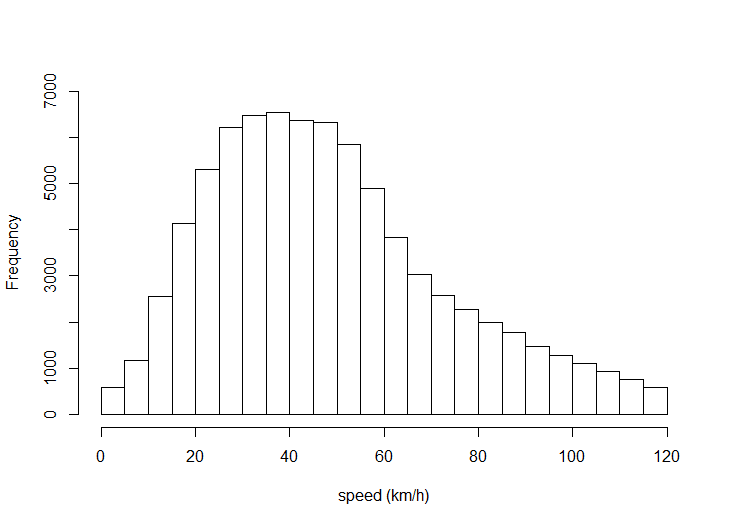
\includegraphics[width=0.7\textwidth]{figures/avg_speed_green_class_matched}}
	{}

\paragraph{Map matching}

Using a MATSim adapted version of Graphhopper, the trip legs are matched to the MATSim road network.
A Hidden Markov Model \citep{newson2009hidden} identifies canditate links for each GPS point, with a measurement sigma of 50m.
An unlimited distance between consecutive points is allowed.
The Graphhopper routing engine then identifies the best route from the set of candidate links.
A minimum of two matched GPS points are required.
The map matching module returns a list of links thier matched GPS points.

\paragraph{Link entry and exit time calculation}
To convert the GPS traces to MATSim events and calculate externalities, the travel time for each link is required.
This is not calculated by Graphhopper, as the state of the art Hidden Markov Model approach used \citep{newson2009hidden} does not consider speed limits or feasible travel times when identifying candidate links for matching.
In the absence of high-frequency GPS measurements or additional sensor information, there may be insufficient GPS measurements to match every intersection in a trivial manner.
Hence, an algorithm that also handles links where few or no GPS measurements are available has been developed for determining this.

A trip leg contains a sequence of links $L$ with the set of GPS points $P(l)$ matched to each link $l$.
For convenience, let the first and last GPS point on each link in the set $L$ be $p_{l,s}$ and $p_{l,e}$ respectively.
The start and end links of a trip leg always have at least one GPS point associated with them, while other links may have none or more GPS points.
Hence, trip legs are divided into sets of consecutive links  $L'$, beginning at $l'_1$,  where $l'_{2..k}$ have no GPS points.
The GPS recorded travel time over the links in $L'$ is then proportionally allocated based on the freespeed travel time of each link $L'$, where $l_{k+1}$ is the next non-empty link.

Let the projection of GPS point $p_{l,i}$ onto link $l$ be $p'_{l,i}$.
A helper function $time\_between(a,b)$ returns the time needed to travel between projected points and verticies of a link.
From $p'_{l,e}$ to the end of a link; or the start of a link to the first projected point on a link $p'_{l,s}$.
$tt(l)$ gives the time needed to travel a link under free flow conditions, and $time_between(p_{l,e}, p_{l',s}$) gives the time difference between the last and first points on two links respectively.

In MATSim, the assumptions hold that an agent always starts and ends somewhere on a link.
Hence, only the exit time for the first link and the entry time for the last link need to be calculated.
Additionally, $entry\_time(l_{j}) = exit\_time(l_{j-1}),  \forall j = 1..n$.
As such, the algorithm can be separated into two cases:
\begin{itemize}
	\item \textbf{First Link} For the first link $l_1$, $exit\_time(l_1) = time(p'_{l_1,e}) + time\_between(p'_{l_1,e}, l_1)$
%%%	\item \textbf{Last Link} For the last link $l_n$, $entry\_time(l_n) = exit\_time(l_{n-1}) + time\_between(l_{n-1}, p'_{l_n,s})$
	\item \textbf{Other Links} \\
		$entry\_time(l_{j}) = exit\_time(l_{j-1}) $ \\
		\textbf{if} $P(l_j) = \emptyset$ \textbf{then} $exit\_time(l_j) = entry\_time(l_j) + 
										\frac{length(l_j) \cdot time\_between(p'_{l_{j-1},e}, p'_{l_{j+k},s})}{distance(p'_{l_{j-1},e}, p'_{l_{j+k},s})} $ \\
										\t where $l_{k}$ is the next successive link with $P(l_k) \neq \emptyset$  \\
		\textbf{else}  $exit\_time(l_j) = entry\_time(l_j) + time\_between(l_{j}, p'_{l_j,e}) + \frac{time\_between(p'_{l_j,e}, l_{j}) \cdot time\_between(p'_{l_j,e}, p'_{l_{j+1},s})} 
					{time\_between(p'_{l_j,e}, l_{j}) + time\_between(l_{j+1},p'_{l_{j+1},s})}   $ \\
\end{itemize}

\paragraph{Conversion to MATSim events} 
The sequence of links with entry and exit times are then converted to valid MATSim events and grouped by person and date.

\paragraph{Imputation of externalities on MATSim events}
To impute the externalities of each trip leg, the events are processed using a MATSim framework set up with two additional modules.
The first, developed by \citet{kaddoura2017simulation} calculates the emitted pollutant amounts inccured on each link, based on the observed travel speed.
Values and emissions factors are taken from the HBEFA database (version 3.2).
Average speeds on each link are capped at the link freespeed.
The road types for assigning emissions factors are taken from OSM.
Each driver is assigned a medium sized vehicle with a 4-cylinder EURO-4 compliant petrol engine.
It was not possible at this stage to represent the actual owned vehicles of the study participants.

For congestion, the caused delays per link are imputed from the average hourly values calculated from the MATSim scenario.
The time lost per link is defined as the difference between the link travel time and travel time under free flow conditions.
From here, it is straightforward to determine the total generated pollution and caused and experienced delay per trip leg.
